%% abtex2-modelo-projeto-pesquisa.tex, v-1.9.6 laurocesar
%% Copyright 2012-2016 by abnTeX2 group at http://www.abntex.net.br/ 
%%
%% This work may be distributed and/or modified under the
%% conditions of the LaTeX Project Public License, either version 1.3
%% of this license or (at your option) any later version.
%% The latest version of this license is in
%%   http://www.latex-project.org/lppl.txt
%% and version 1.3 or later is part of all distributions of LaTeX
%% version 2005/12/01 or later.
%%
%% This work has the LPPL maintenance status `maintained'.
%% 
%% The Current Maintainer of this work is the abnTeX2 team, led
%% by Lauro César Araujo. Further information are available on 
%% http://www.abntex.net.br/
%%
%% This work consists of the files abntex2-modelo-projeto-pesquisa.tex
%% and abntex2-modelo-references.bib
%%

% ------------------------------------------------------------------------
% ------------------------------------------------------------------------
% abnTeX2: Modelo de Projeto de pesquisa em conformidade com 
% ABNT NBR 15287:2011 Informação e documentação - Projeto de pesquisa -
% Apresentação 
% ------------------------------------------------------------------------ 
% ------------------------------------------------------------------------

\documentclass[
	% -- opções da classe memoir --
	12pt,				% tamanho da fonte
%	openright,			% capítulos começam em pág ímpar (insere página vazia caso preciso)
	openany,
%	twoside,			% para impressão em recto e verso. Oposto a oneside
	oneside,
	a4paper,			% tamanho do papel. 
	% -- opções da classe abntex2 --
	%chapter=TITLE,		% títulos de capítulos convertidos em letras maiúsculas
	%section=TITLE,		% títulos de seções convertidos em letras maiúsculas
	%subsection=TITLE,	% títulos de subseções convertidos em letras maiúsculas
	%subsubsection=TITLE,% títulos de subsubseções convertidos em letras maiúsculas
	% -- opções do pacote babel --
	english,			% idioma adicional para hifenização
	brazil,				% o último idioma é o principal do documento
	]{abntex2}

% ---
% PACOTES
% ---

% ---
% Pacotes fundamentais 
% ---
\usepackage{lmodern}			% Usa a fonte Latin Modern
\usepackage[T1]{fontenc}		% Selecao de codigos de fonte.
\usepackage[utf8]{inputenc}		% Codificacao do documento (conversão automática dos acentos)
\usepackage{indentfirst}		% Indenta o primeiro parágrafo de cada seção.
\usepackage{color}				% Controle das cores
\usepackage{graphicx}			% Inclusão de gráficos
\usepackage{microtype} 			% para melhorias de justificação
% ---

% ---
% Pacotes adicionais, usados apenas no âmbito do Modelo Canônico do abnteX2
% ---
\usepackage{lipsum}				% para geração de dummy text
% ---

% ---
% Pacotes de citações
% ---
\usepackage[brazilian,hyperpageref]{backref}	 % Paginas com as citações na bibl
\usepackage[alf]{abntex2cite}	% Citações padrão ABNT




\usepackage{graphicx}
\usepackage{enumerate}
\usepackage{float}


\graphicspath{{figuras/}}








% --- 
% CONFIGURAÇÕES DE PACOTES
% --- 

% ---
% Configurações do pacote backref
% Usado sem a opção hyperpageref de backref
\renewcommand{\backrefpagesname}{Citado na(s) página(s):~}
% Texto padrão antes do número das páginas
\renewcommand{\backref}{}
% Define os textos da citação
\renewcommand*{\backrefalt}[4]{
	\ifcase #1 %
		Nenhuma citação no texto.%
	\or
		Citado na página #2.%
	\else
		Citado #1 vezes nas páginas #2.%
	\fi}%
% ---

% ---
% Informações de dados para CAPA e FOLHA DE ROSTO
% ---
\titulo{Um sistema para auxiliar na\\ aprendizagem da disciplina\\ Linguagens Formais e Autômatos}
\autor{Rafael Cardoso da Silva}
\local{Santo André - SP, Brasil}
\data{2016}
\instituicao{%
  Universidade Federal do ABC -- UFABC
  \par
  Bacharelado em Ciências e Tecnologia
  \par
  Projeto Dirigido}
\tipotrabalho{Projeto de Pesquisa}
% O preambulo deve conter o tipo do trabalho, o objetivo, 
% o nome da instituição e a área de concentração 
\preambulo{Projeto de pesquisa apresentado à Disciplina de Projeto Dirigido do curso de Bacharelado de Ciência e Tecnologia..}
% ---

% ---
% Configurações de aparência do PDF final

% alterando o aspecto da cor azul
\definecolor{blue}{RGB}{41,5,195}

% informações do PDF
\makeatletter
\hypersetup{
     	%pagebackref=true,
		pdftitle={\@title}, 
		pdfauthor={\@author},
    	pdfsubject={\imprimirpreambulo},
	    pdfcreator={LaTeX with abnTeX2},
		pdfkeywords={autômato finito}{equivalência de autômatos}{minimização de autômato}{programação para web}, 
		colorlinks=false,       		% false: boxed links; true: colored links
    	linkcolor=blue,          	% color of internal links
    	citecolor=blue,        		% color of links to bibliography
    	filecolor=magenta,      	% color of file links
		urlcolor=blue,
		bookmarksdepth=4
}
\makeatother
% --- 

% --- 
% Espaçamentos entre linhas e parágrafos 
% --- 

% O tamanho do parágrafo é dado por:
\setlength{\parindent}{1.3cm}

% Controle do espaçamento entre um parágrafo e outro:
\setlength{\parskip}{0.2cm}  % tente também \onelineskip

% ---
% compila o indice
% ---
\makeindex
% ---

% ----
% Início do documento
% ----
\begin{document}

% Seleciona o idioma do documento (conforme pacotes do babel)
%\selectlanguage{english}
\selectlanguage{brazil}

% Retira espaço extra obsoleto entre as frases.
\frenchspacing 

% ----------------------------------------------------------
% ELEMENTOS PRÉ-TEXTUAIS
% ----------------------------------------------------------
% \pretextual

% ---
% Capa
% ---
\imprimircapa
% ---

% ---
% Folha de rosto
% ---
\imprimirfolhaderosto
% ---

% ---
% NOTA DA ABNT NBR 15287:2011, p. 4:
%  ``Se exigido pela entidade, apresentar os dados curriculares do autor em
%     folha ou página distinta após a folha de rosto.''
% ---

% ---
% inserir lista de ilustrações
% ---
%\pdfbookmark[0]{\listfigurename}{lof}
%\listoffigures*
%\cleardoublepage
% ---

% ---
% inserir lista de tabelas
% ---
%\pdfbookmark[0]{\listtablename}{lot}
%\listoftables*
%\cleardoublepage
% ---

% ---
% inserir lista de abreviaturas e siglas
% ---
%\begin{siglas}
%  \item[ABNT] Associação Brasileira de Normas Técnicas
%  \item[abnTeX] ABsurdas Normas para TeX
%\end{siglas}
% ---

% ---
% inserir lista de símbolos
% ---
%\begin{simbolos}
%  \item[$ \Gamma $] Letra grega Gama
%  \item[$ \Lambda $] Lambda
%  \item[$ \zeta $] Letra grega minúscula zeta
%  \item[$ \in $] Pertence
%\end{simbolos}
% ---

% ---
% inserir o sumario
% ---
\pdfbookmark[0]{\contentsname}{toc}
\tableofcontents*
%\cleardoublepage
% ---


% ----------------------------------------------------------
% ELEMENTOS TEXTUAIS
% ----------------------------------------------------------
\textual

%\begin{resumo}
\chapter*[Resumo]{Resumo}
 \noindent Resolver exercícios é fundamental para um aluno fixar os conceitos apresentados em aula. Por outro lado, ter seus exercícios corrigidos também é muito importante, para que ele possa avaliar o seu aprendizado. Na UFABC, a disciplina de Linguagens Formais e Autômatos contempla vários exercícios que admitem infinitas respostas, o que torna a correção deles praticamente impossível, principalmente quando as turmas são grandes. O objetivo deste projeto é a criação e implementação de um sistema para aplicação e correção automática de exercícios envolvendo autômatos finitos determinísticos. Através do estudo de métodos e algoritmos presentes na literatura, será possível implementar o teste de equivalência entre o autômato-resposta do aluno e o autômato-gabarito previamente armazenado no banco de dados. E ao final do projeto, o sistema será utilizado em caráter experimental numa turma da UFABC da disciplina de Linguagens Formais e Autômatos, afim de testar a sua qualidade. E ao final da disciplina, a nota que os alunos obterão ao revolver os exercícios do sistema ajudarão a compor o conceito final de cada um na disciplina.

\bigskip

\noindent\textbf{Palavras-chave}: autômato finito, equivalência de autômatos, minimização de autômato, programação para web.


\chapter{Introdução}

	Resolução de exercícios é uma atividade fundamental para que um aluno possa praticar o que foi apresentado em aula. A correção dos exercícios também é importante para que o aluno possa avaliar seu aprendizado. Para turmas grandes, torna-se inviável corrigir rapidamente todos os exercícios propostos e devolvê-los em tempo hábil aos alunos. Na disciplina MC3106 – Linguagens Formais e Autômatos – vários exercícios da parte inicial da disciplina pedem como resposta um autômato finito determinístico. Tais exercícios são particularmente trabalhosos de se corrigir porque cada um deles admite infinitas respostas corretas e, por esse motivo, sua correção se torna exaustiva para o monitor ou docente responsável.
	
	Com o intuito de agilizar essa tarefa, este projeto propõe o desenvolvimento de um sistema web que permita ao aluno inserir seu autômato-resposta por meio de uma interface intuitiva e fácil de ser utilizada e obter um \emph{feedback} quase que imediatamente, um tempo drasticamente reduzido se comparado à correção manual. Acreditamos que um sistema como esse será de grande valia para o aprendizado dos alunos. Por outro lado, para o docente responsável, facilitará o processo de composição do conceito final na disciplina de Linguagens Formais e Autômatos.


\chapter[O Principal Problema]{O Principal Problema}

Um \emph{autômato finito determinístico} (também chamado de AFD ou máquina de estados) consiste de um conjunto de estados não vazio $Q$, um alfabeto $\Sigma$, um estado inicial $s \in Q$, um conjunto de estados de aceitação $F \subseteq Q$ e uma função de transição $\delta \colon Q \times \Sigma \rightarrow Q$. É comum estender a função de transição para uma função $\hat{\delta} \colon Q \times \Sigma^* \rightarrow Q$ definida indutivamente por
\begin{alineas}%[(i)]
	\item[(i)] $\hat{\delta}(q, \varepsilon) = q$ para todo estado $q \in Q$;
	\item[(ii)] $\hat{\delta}(q, \sigma) = \delta(q, \sigma)$ para todo estado $q \in Q$ e símbolo $\sigma \in \Sigma$;
	\item[(iii)] $\hat{\delta}(q, \sigma_1 \cdots \sigma_k) = \delta(\hat{\delta}(q, \sigma_1 \cdots \sigma_{k-1}), \sigma_k)$ para todo estado $q \in Q$ e símbolos $\sigma_1, \dots, \sigma_k \in \Sigma$.
\end{alineas}



Todo autômato pode ser representado por um diagrama de estados. Considere o diagrama da Figura~\ref{fig:aut01} abaixo.

\begin{figure}[H]
	\vspace{-0.4cm}
	\centering
	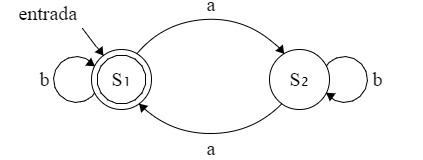
\includegraphics[scale=0.75]{aut01.png}
	\vspace{-0.5cm}
	\caption{Um autômato $M_1$.}
	\label{fig:aut01}
	\vspace{-0.5cm}
\end{figure}


No autômato da Figura~\ref{fig:aut01}, temos $Q = \{S_1, S_2\}$, $\Sigma = \{a, b\}$, $s = S_1$, $F = \{S_1\}$ e a função de transição  é dada pela tabela a seguir.

\begin{table}[H]
	\centering
	\begin{tabular}[H]{c|c c}
		$\delta$ & \textbf{\texttt{a}} & \textbf{\texttt{b}} \\
		\hline
		$S_1$    & $S_2$               & $S_1$               \\
		$S_2$    & $S_1$               & $S_2$
	\end{tabular}
	\caption{Tabela de transições do $M_1$.}
	\label{tab:tabTransicoesM1}
	\vspace{-0.5cm}
\end{table}


Nesse exemplo, se o AFD $M_1$ é alimentado com a palavra \textbf{\texttt{aabab}}, ele irá começar no estado $S_1$ e irá percorrer os estados $S_2$, $S_1$, $S_1$, $S_2$, $S_2$ nesta ordem, e irá rejeitar a palavra dada (pois o último estado $S_2 \not\in F$). Se, para uma outra palavra $w$, a simulação tivesse terminado em $S_1$ (que pertence a $F$) =íamos que o autômato aceita a palavra $w$. Mais formalmente, se $M_1 = (Q, \Sigma, \delta, s, F)$ é um autômato finito determinístico, dizemos que $M_1$ \emph{aceita} $w$ se $\hat{\delta}(s, w) \in F$ e que $M_1$ \emph{rejeita} $w$ caso contrário.

A \emph{linguagem reconhecida} por um autômato $M_1 = (Q, \Sigma, \delta, s, F)$ é o conjunto de palavras que são aceitas por esse autômato, ou seja, é definida pelo conjunto $ L(M_1) = \{w \in \Sigma^* \colon \hat{\delta}(s, w) \in F \}$. No exemplo da Figura~\ref{fig:aut01} acima, a linguagem reconhecida por por $M_1$ é $L(M_1) = \{w \in \Sigma^* :  w$  tem número par de símbolos $\mathtt{a}\}$.

\bigskip

Vários tipos de exercícios pedem por uma resposta que é um autômato. Por exemplo:
\begin{alineas}%[(i)]
	\item[(i)] construir um autômato que reconheça a linguagem regular
	dada por um certo conjunto de palavras descrito matematicamente;
	\item[(ii)] transformar um autômato finito não determinístico num
	determinístico equivalente;
	\item[(iii)] criar um autômato que reconheça a mesma linguagem
	descrita por uma expressão regular dada;
	\item[(iv)] construir o menor autômato finito determinístico
	que reconheça uma certa linguagem regular.
\end{alineas}

Cada um destes tipos de exercícios possui centenas de casos particulares que os alunos podem fazer para praticar os conceitos de autômatos abordados na disciplina. Tais exercícios podem, por exemplo, ser encontrados abundantemente no livro \textit{Introdução à Teoria da Computação} de M. Sipser~\cite{sipser}. Outras referências importantes da disciplina que possuem exercícios semelhantes são~\cite{ullman} e~\cite{linz}. Em todos os casos acima, contudo, há uma infinidade de respostas corretas para cada exercício. Por exemplo, considere o diagrama abaixo.

\begin{figure}[H]
	\vspace{-0.5cm}
	\centering
	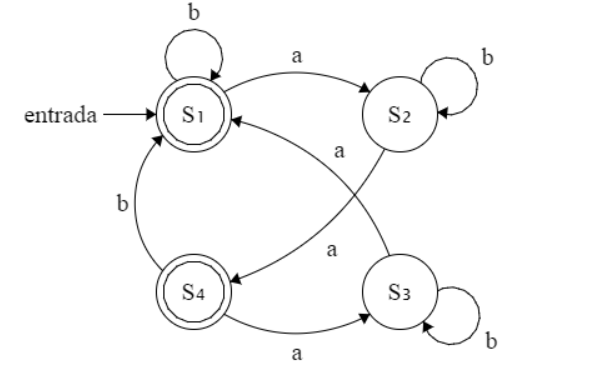
\includegraphics[scale=.65]{aut02.png}
	\vspace{-0.2cm}
	\caption{Um autômato $M_2$.}
	\label{fig:aut02}
	\vspace{-0.5cm}
\end{figure}

Apesar de visivelmente maior e mais complexo que $M_1$, este autômato reconhece a mesma linguagem que o autômato $M_1$ da Figura~\ref{fig:aut01}. É possível demonstrar que, para cada linguagem regular, existem infinitos autômatos que a reconhecem. Como decidir então se o autômato-resposta dado por um aluno reconhece a linguagem pedida? No caso do sistema que iremos desenvolver isso se reduz ao seguinte problema:
\bigskip

{\large
\noindent \textbf{Problema:} Decidir se dois autômatos finitos determinísticos reconhecem a mesma linguagem.
}


\section {Breve descrição do método}

Determinar se dois autômatos finitos e determinísticos reconhecem linguagens diferentes é um problema bem resolvido. A idéia fundamental é tentar encontrar uma palavra~$w$ que é aceita por um autômato e rejeitada pelo outro. Se tal palavra puder ser encontrada, então as linguagens reconhecidas por esses autômatos são distintas. Caso tal palavra não exista, os autômatos reconhecem a mesma linguagem. 

Mais formalmente, dizemos que dois estados $q_1$ e $q_2$ (no mesmo autômato ou não) são \emph{equivalentes} se, para toda palavra~$w \in \Sigma^*$ vale que $\hat{\delta}(q_1, w) \in F$ se e somente se $\hat{\delta}(q_2, w) \in F$. Dois autômatos serão, portanto, equivalentes se e somente se seus respectivos estados iniciais forem equivalentes no sentido que acabamos de definir.

Esse problema está intimamente relacionado com o problema de minimização de autômatos finitos determinísticos. Os primeiros algoritmos desenvolvidos para testar a equivalência de autômatos resolviam também o problema da minimização. Eles apareceram em~\cite{huffman} e~\cite{moore} e podem ser implementados sem muito esforço em tempo~$O(n^2)$, onde~$n$ é o número total de estados. O algoritmo mais eficiente conhecido para minimização de autômatos~\cite{hopcroft} executa em tempo~$O(n \log{n})$. Posteriormente Hopcroft e Karp~\cite{hopcroft_karp} desenvolveram um algoritmo linear para testar a equivalência de autômatos.

%Com a finalidade de contemplar uma maior variedade de exercícios e abranger uma fração maior do conteúdo coberto na disciplina MC3106, seria interessante se nosso sistema pudesse aceitar, como resposta para alguns exercícios, um autômato finito não determinístico (AFN) ou uma expressão regular. No entanto, determinar se dois AFNs (ou duas expressões regulares) são equivalentes é um problema \textsc{PSPACE}-completo (veja problema AL01 de~\cite{garey79}) e, portanto, muito difícil computacionalmente. Contudo, para um AFN-resposta não muito grande (até 25 estados) seria viável construir um AFD equivalente para que o algoritmo de Hopcroft e Karp pudesse então verificar se ele é equivalente ao AFD-gabarito armazenado no banco de dados do servidor.

%Neste projeto o aluno implementará todos os algoritmos envolvidos na discussão acima como parte de um sistema maior que descrevemos na próxima seção.

Neste projeto será implementado todos os algoritmos envolvidos na discussão acima como parte de um sistema maior que descrevemos na próxima seção.





\section {Breve descrição do sistema}

Como mencionamos anteriormente, a proposta deste projeto é a criação de um site que disponibilize uma lista de exercícios aos usuários -- que serão os alunos da disciplina MC3106 -- e que permita a correção automática desses exercícios. Esse site será semelhante aos sistemas de correção automática utilizados em eventos de maratona de programação, onde o competidor submete sua respostar para resolução de algum problema proposto, e o sistema analisa a resposta recebida e dá um retorno da submissão. Em nosso sistema, por meio de uma interface intuitiva, o usuário poderá ver a lista de exercícios e, para cada um deles, poderá consultar o seu estado: se ainda não foi resolvido, se há um rascunho de resposta salvo, se uma resposta já foi submetida, e qual foi o conceito ou \emph{feedback} devolvido ao aluno em cada submissão.

Ao clicar num exercício especifico, o aluno verá uma página com o título do exercício, o corpo do texto com a descrição do exercício que o ele deve resolver, e uma área dedicada para a confecção da resposta-autômato. Para a confecção desta resposta, usaremos como front-end um JavaScript desenvolvido e disponibilizado por Evan Wallace~\cite{evan} sob a licença MIT~\cite{mit} que, de maneira muito simples e intuitiva, permite a construção de diagramas de máquina de estados.

O aluno então resolve o exercício da maneira tradicional e concebe um autômato como possível resposta. Em seguida ele poderá, com o auxílio do mouse e do teclado, inserir o diagrama de seu autômato no espaço designado, alterando-o quantas vezes achar necessário. O aluno tem a opção de salvar seu trabalho para continuar mais tarde e também de submetê-lo como resposta. Quando ele decidir submeter, a estrutura do autômato construído pelo aluno nesta interface será validada (por um script que decide se o diagrama construído é de fato um AFD) e será enviada para o servidor.

No servidor, será executado o programa que será implementado pelo bolsista com o algoritmo de Hopcroft e Karp para testar a equivalência de autômatos finitos determinísticos. Se o autômato que o aluno construiu for equivalente ao AFD-gabarito armazenado no banco de dados, então o aluno terá resolvido o exercício corretamente. Se não forem equivalentes, podemos encontrar uma palavra que distingue os dois autômatos e enviar essa palavra ao aluno para que ele tenha um \emph{feedback} e um certificado de que sua resposta está incorreta. Examinando essa palavra com mais cuidado, o aluno poderá então perceber a razão pela qual seu autômato não reconhece a linguagem pedida. Ele poderá elaborar uma outra resposta-autômato e fazer uma nova submissão, de acordo com a data final para a submissão de cada exercício determinado previamente pelo administrador.

Do ponto de vista do professor da disciplina, que será um administrador do sistema, pretendemos implementar as seguintes funcionalidades: criação e gerenciamento de turmas, o gerenciamento de listas compostas de exercícios, gerenciamento do banco de questões para compor as listas e, por fim, visualização e exportação da planilha final de notas. 

Para a implementação deste sistema, serão necessários conhecimentos das disciplinas Programação para WEB e Linguagens Formais e Autômatos, que o aluno proponente deste projeto já cursou na UFABC. Se houver tempo, confeccionaremos ainda outras ferramentas para correção automática de outras classes de exercícios que a disciplina engloba e faremos a integração com o sistema. 



\chapter {Objetivos}

%\section {Gerais:}

%\noindent 
Os Objetivos Gerais deste projeto são os seguintes:

\begin{alineas}
	\item[$\bullet$] Incentivar o gosto do bolsista pela pesquisa aplicada.
	\item[$\bullet$] Desenvolver a maturidade do aluno em tópicos centrais de ciência da computação.
	\item[$\bullet$] Incentivar e aprimorar as habilidades de programação do candidato.
	\item[$\bullet$] Envolver o aluno em um projeto com fins de ensino e aprendizagem.
\end{alineas}

%\section {Específicos:}

%\noindent 
Os Objetivos Específicos são que o aluno implemente:

\begin{alineas}
	\item[$\bullet$] o algoritmo de Moore para minimização e equivalência de AFDs;
	\item[$\bullet$] o algoritmo de Hopcroft para minimização de AFD;
	\item[$\bullet$] o algoritmo de Hopcroft e Karp para testar a equivalência de AFDs;
%	\item o algoritmo que transforma uma expressão regular num AFN;
%	\item o algoritmo que transforma um AFN num AFD;
%	\item um algoritmo envolvendo gramáticas livres de contexto (se o tempo permitir).
\end{alineas}

Todos os itens citados fazem parte da finalidade deste projeto de implementar o sistema descrito, algo que também envolve implementações de programas em JavaScript e C/C++ além de outras linguagens e tecnologias envolvidas na interface cliente/servidor como HTMl, PHP, MySQL, etc.

\chapter{Metodologia}

Este projeto será conduzida da seguinte forma. Num período inicial o aluno se preocupará em ler as seções relevantes das referências~\cite{sipser},~\cite{ullman}~e~\cite{linz}, a fim de criar familiaridade com o problema de equivalência, e abstrair os conceitos iniciais do algoritmo de minimização de autômatos finitos determinísticos. Será uma revisão de tópicos cobertos na disciplina de Linguagens Formais e Autômatos, que o aluno já cursou na UFABC.   

Passada a fase inicial, o aluno aprofundará seus estudos nos artigos~\cite{hopcroft} e~\cite{hopcroft_karp} que descrevem os algoritmos mais eficientes para minimização e equivalência de autômatos respectivamente.  À medida que o aluno for conhecendo os melhores algoritmos para cada problema, ele irá implementar o sistema, aplicando os conceitos e os algoritmos estudados. Uma outra parte considerável do projeto será dedicada a elaboração e compilação de exercícios (populando um banco de dados e/ou possivelmente elaborando scripts que geram exercícios automaticamente) e aos testes do sistema para que ele possa ser usado na UFABC já com a primeira turma de MC3106 após o término deste projeto.  

O orientador irá acompanhar seu progresso em reuniões semanais, quando o aluno esclarecerá suas dúvidas e o orientador poderá complementar a formação do bolsista explicando-lhe conceitos pertinentes que possivelmente não estejam cobertos nos livros e artigos indicados anteriormente, bem como apontar novos artigos relevantes sobre o assunto e indicar direções que devam ser seguidas na implementação do sistema.  



\chapter{Cronograma}

O bolsista deverá dedicar a este projeto um mínimo de 20 horas por semana. O projeto irá se desenrolar conforme os itens abaixo:  

\begin{alineas}
%	\item Leitura da bibliografia (capítulos de livros e artigos citados).
%	\item Implementação dos algoritmos que decidem a equivalência de dois AFDs em C/C++.
%	\item Implementação dos algoritmos de minimização de AFD (para armazenamento econômico dos gabaritos) em C/C++.
%	\item Design e construção do banco de dados de exercícios e gabaritos.
%	\item Adequação do script de Evan Wallace às necessidades deste projeto.
%	\item Implementação dos algoritmos que convertem uma expressão regular num AFN e um AFN num AFD.
%	\item Elaboração do relatório parcial.
%	\item Sistema de criação e gerenciamento de usuários.
%	\item Sistema de logs de submissões.
%	\item Finalização da versão para testes.
%	\item Elaboração do relatório final.

	\item[1.] Leitura da bibliografia (capítulos de livros e artigos citados).
	\item[2.] Implementação dos algoritmos em C++.
	\item[3.] Adequação do FSM Designer às necessidades deste projeto.
    \item[4.] Desenvolvimento do sistema.
	\begin{alineas}
		\item[4.1.] Levantamento de requisitos, análise e projeto do sistema.
		\item[4.2.] Implementação do sistema.
	\end{alineas}
	\item[5.] Confecção dos exercícios no sistema.
	\item[6.] Aplicação numa turma experimental.
	\item[7.] Elaboração do relatório final.
\end{alineas}


O andamento do projeto se dará conforme a Tabela~\ref{tab:cronograma} abaixo (os números à esquerda indicam as tarefas enumeradas na seção anterior). 

\begin{table}[H]
\caption{Cronograma}
\centering
	\begin{tabular}{|l||c|c|c|c|c|c|c|c|c|c|c|c|}
		\hline 
%		   & 1º & 2º & 3 & 4º & 5º & 6º & 7º & 8º & 9º & 10º & 11º & 12º \\ 
		   &ago&set&out&nov&dez&jan&fev&mar&abr&mai&jun&jul\\
		\hline 
		1  & x & x & x & x & x & x & x &  &  &  &  &  \\ 
		2  & x & x & x & x &  &  &  &  &  &  &  &  \\ 
		3  &  &  &  & x & x &  &  &  &  &  &  &  \\ 
		4  &  &  &  &  &  & x & x & x & x & x &  &  \\ 
		4.1  &  &  &  &  &  & x &  &  &  &  &  &  \\ 
		4.2  &  &  &  &  &  &  & x & x & x & x &  &  \\ 
		5 &  &  &  &  &  &  &  &  & x & x &  &  \\ 
		6  &  &  &  &  &  &  &  &  &  & x & x & x \\ 
		7 &  &  &  &  &  &  &  &  & x & x & x & x \\ 
		\hline 
	\end{tabular} 
\label{tab:cronograma}
\end{table}


%\begin{table}[H]
%	\caption{Cronograma}
%	\centering
%	\begin{tabular}{|c||c|c|c|c|c|c|c|c|c|c|c|c|}
%		\hline
%		&ago&set&out&nov&dez&jan&fev&mar&abr&mai&jun&jul\\
%		\hline\hline
%		\textbf{1}  & x & x & x & x & x & x & x & x &   &   &   &   \\ % pesquisa bibliográfica
%		\textbf{2}  &   & x & x &   &   &   &   &   &   &   &   &   \\ % equivalência de AFDs
%		\textbf{3}  &   &   & x & x &   &   &   &   &   &   &   &   \\ % minimizacao AFD
%		\textbf{4}  &   &   &   & x & x & x & x & x & x &   &   &   \\ % banco de exercícios
%		\textbf{5}  &   &   &   &   & x & x &   &   &   &   &   &   \\ % adaptar script do E. Wallace
%		\textbf{6}  &   &   &   &   & x & x &   &   &   &   &   &   \\ % algoritmos de conversão
%		\textbf{7}  &   &   &   &   &   & x & x &   &   &   &   &   \\ % relat parc
%		\textbf{8}  &   &   &   &   &   &   &   & x & x &   &   &   \\ % sistema de usuários
%		\textbf{9}  &   &   &   &   &   &   &   &   & x & x &   &   \\ % sistema para log de submissões
%		\textbf{10} &   &   &   &   &   &   &   &   &   & x & x & x \\ % testes e finalização
%		\textbf{11} &   &   &   &   &   &   &   &   &   & x & x & x \\ % relat final
%		\hline
%	\end{tabular}
%	\label{tableSS2}
%\end{table}


%O projeto será avaliado de acordo com os seguintes critérios:

%\begin{alineas}
%	\item[(a)] desempenho do bolsista;
%	\item[(b)] adequação das atividades ao cronograma proposto.
%\end{alineas}




\chapter{Orçamento do Pesquisa}

O Orçamento para a execução deste projeto pode ser vista pela tabela a abaixo.
\begin{table}[H]
  \caption{Orçamento}
  \centering
  \begin{tabular}{|r l|l|}
    \hline 
    \multicolumn{3}{|c|}{\textsc{CUSTEIO}} \\ 
    \hline 
    \multicolumn{3}{|l|}{\textbf{Serviços de Terceiro}} \\ 
    \hline 
    (5 meses) & Hospedagem do Site & R\$ 74,50 (R\$ 14,90* cada mês) \\ 
    \hline 
    (1 ano) & Registro de Domínio & R\$ 49,90*   \\ 
    \hline 
    \multicolumn{3}{|c|}{~} \\ 
    \hline 
    \multicolumn{2}{|l|}{\textbf{TOTAL}} & R\$ 124,40\\ 
    \hline 
  \end{tabular} 
  \label{tab:orcamento}
\end{table}

\noindent * valores obtidos com base nos pacotes oferecidos no site da empresa LocaWeb\footnote{Acessado dia 29/10/2016, disponível em \url{http://www.locaweb.com.br/hospedagem-de-sites/}}.



% ----------------------------------------------------------
% ELEMENTOS PÓS-TEXTUAIS
% ----------------------------------------------------------
%\postextual

% ----------------------------------------------------------
% Referências bibliográficas
% ----------------------------------------------------------
\bibliography{pd_latex}

% ----------------------------------------------------------
% Glossário
% ----------------------------------------------------------
%
% Consulte o manual da classe abntex2 para orientações sobre o glossário.
%
%\glossary

% ----------------------------------------------------------
% Apêndices
% ----------------------------------------------------------

% ---
% Inicia os apêndices
% ---
%\begin{apendicesenv}

% Imprime uma página indicando o início dos apêndices
%\partapendices

% ----------------------------------------------------------
%\chapter{Quisque libero justo}
% ----------------------------------------------------------

%\lipsum[50]

% ----------------------------------------------------------
%\chapter{Nullam elementum urna vel imperdiet sodales elit ipsum pharetra ligula
%ac pretium ante justo a nulla curabitur tristique arcu eu metus}
% ----------------------------------------------------------
%\lipsum[55-57]

%\end{apendicesenv}
% ---


% ----------------------------------------------------------
% Anexos
% ----------------------------------------------------------

% ---
% Inicia os anexos
% ---
%\begin{anexosenv}

% Imprime uma página indicando o início dos anexos
%\partanexos

% ---
%\chapter{Morbi ultrices rutrum lorem.}
% ---
%\lipsum[30]

% ---
%\chapter{Cras non urna sed feugiat cum sociis natoque penatibus et magnis dis
%parturient montes nascetur ridiculus mus}
% ---

%\lipsum[31]

% ---
%\chapter{Fusce facilisis lacinia dui}
% ---

%\lipsum[32]

%\end{anexosenv}

%---------------------------------------------------------------------
% INDICE REMISSIVO
%---------------------------------------------------------------------

%\phantompart

%\printindex


\end{document}
